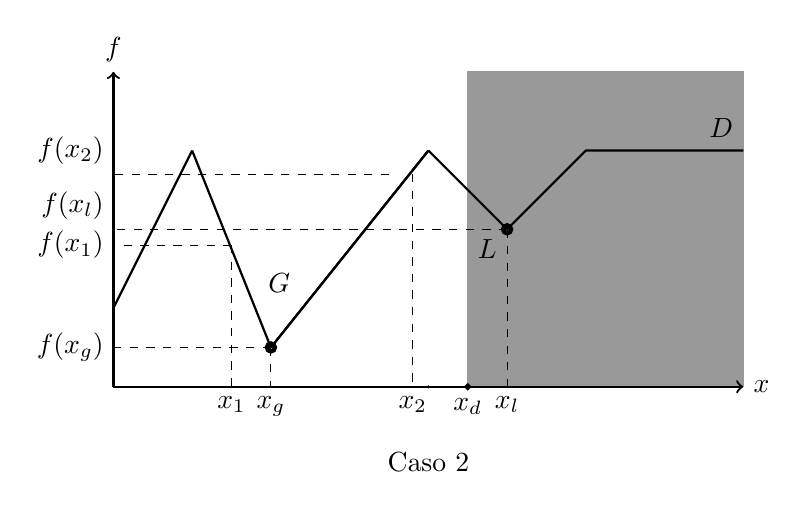
\begin{tikzpicture}
  \draw [->, thick, black] (0,0)--(8,0) node[right] {$x$};
  \draw [->, thick, black] (0,0)--(0,4) node[above] {$f$};
  \draw [thick, black] (0,1)--(1,3);
  \draw [thick, black] (1,3)--(2,0.5) node[above,xshift = 3,yshift = 16] {$G$};
  \draw [thick, black](2,0.5)--(4,3);
  \draw [thick, black](2,0.5)--(4,3);
  \draw [thick, black](4,3)--(5,2) node[below left] {$L$};
  \draw [thick, black](5,2)--(6,3)--(8,3)node[left,yshift=8] {$D$};
  \draw [ultra thick, black](2,0.5) circle (0.5mm);
  \draw [ultra thick, black](4.5,0) circle (0.1mm) node[below]{$x_d$};
  \draw [dashed, black](5,2)--(5,0) node[below] {$x_l$};
  \draw [ultra thick, black](5,2) circle (0.5mm);
  \fill [black, draw=black, opacity = 0.4] (4.5,0) rectangle (8,4);
 %% \draw [thick, black](5,0) circle (0.2mm) node[below] {$x_l$};
  \draw [dashed, black](2,0.5)--(0,0.5) node[left] {$f(x_g)$};
  \draw [dashed, black](2,0.5)--(2,0) node[below] {$x_g$};
  \draw [dashed, black] (1.5,1.8)--(1.5,0) node[below] {$x_1$};
  \draw [dashed, black] (1.5,1.8)--(0.0,1.8) node[left] {$f(x_1)$};
  \draw [dashed, black](3.8,2.7)--(3.8,0) node[below] {$x_2$};
  \draw [dashed, black](3.5,2.7)--(0.0,2.7) node[above left] {$f(x_2)$};
  \draw [dashed, black](5,2)--(0,2) node[above left] {$f(x_l)$};
  \draw [thick, black](4,0) circle (0.01mm) node[below,yshift=-20] {Caso 2};
  \end{tikzpicture}
